\documentclass[]{article}
\usepackage[colorinlistoftodos]{todonotes}
%For front page purposes
\usepackage{pdfpages}
%MISC
\usepackage{framed}
\usepackage{hyperref}
\usepackage{url}
% To handle Icelandic letters
\usepackage[utf8]{inputenc}
\usepackage[T1]{fontenc}


%opening
\title{Like Breeder\\ \small Report in the course Procedural Content Generation in Games, Autumn 2014}
\author{Björn Þór Jónsson and Kasper Fryland Appeldorff}

\begin{document}
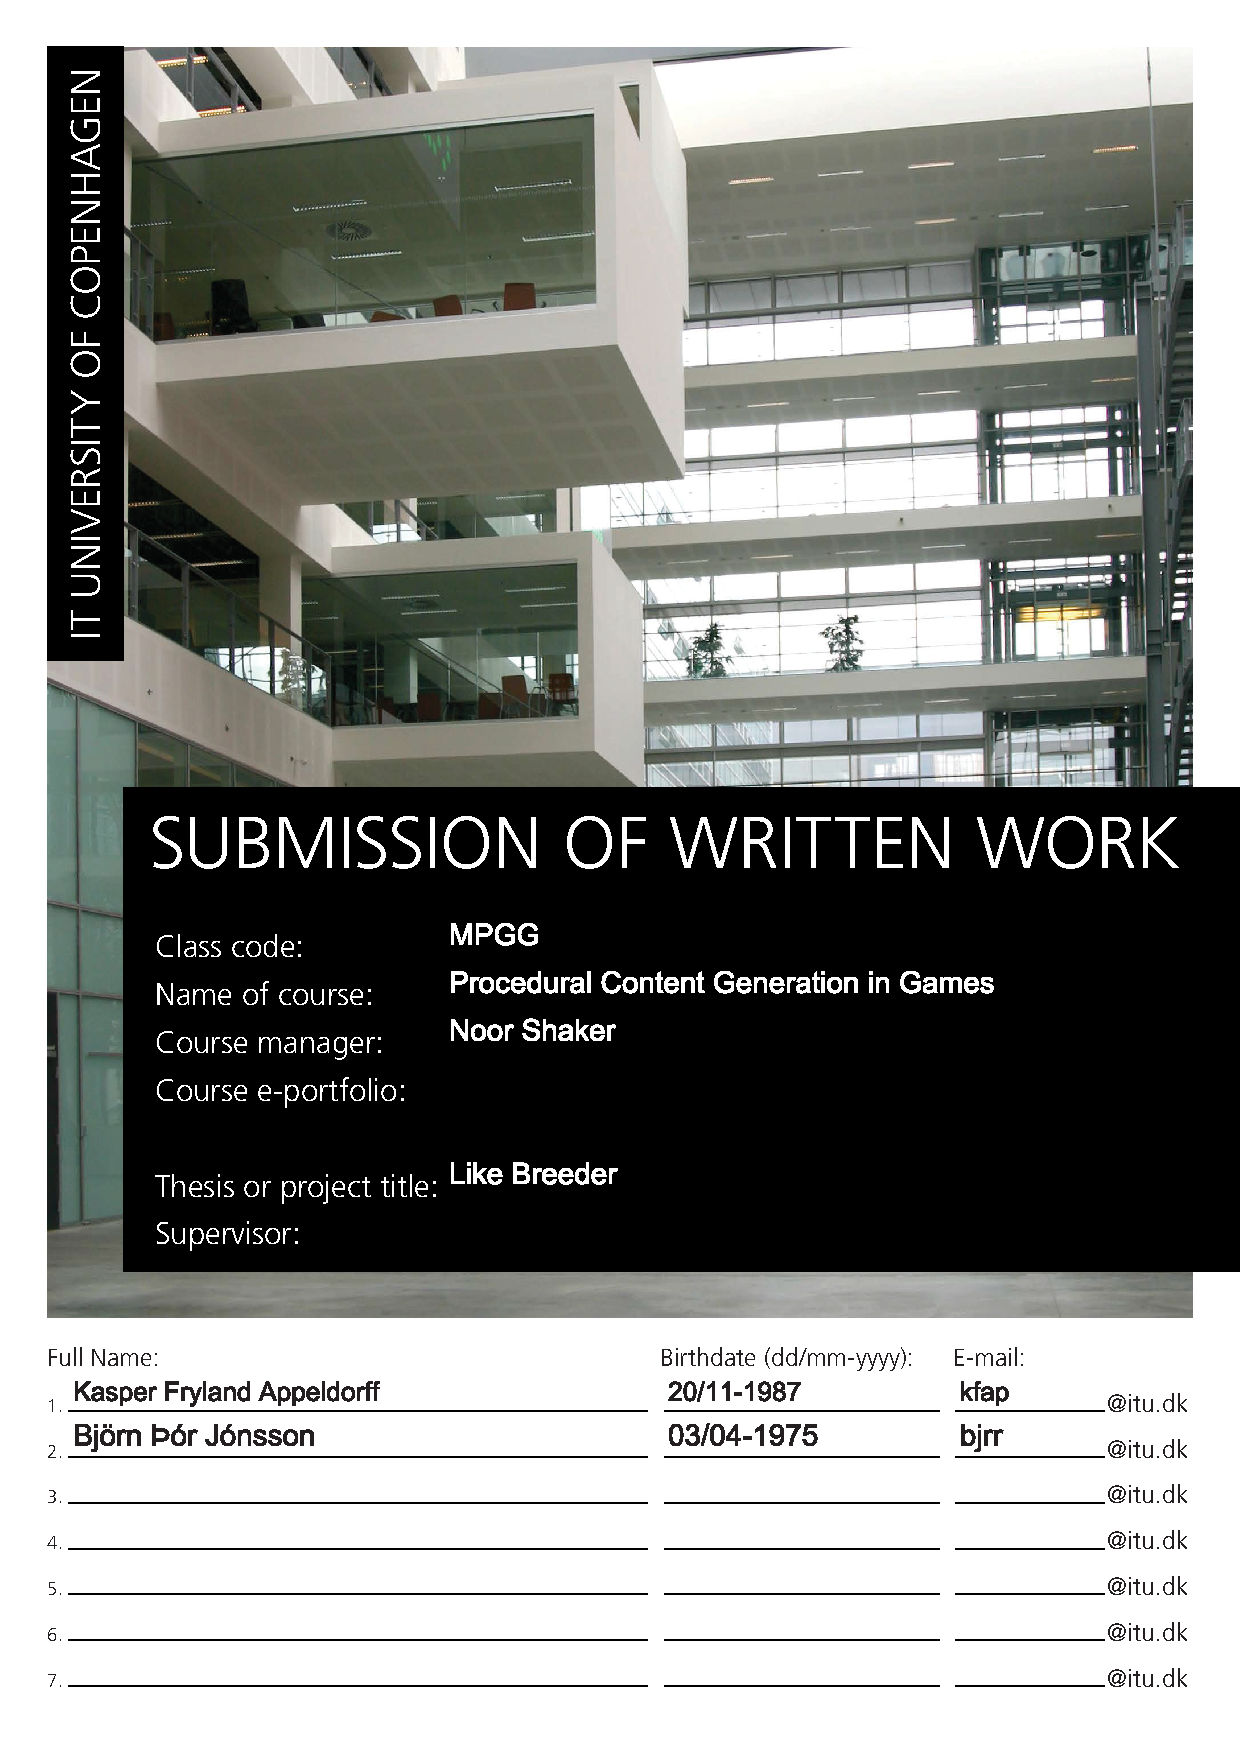
\includepdf{frontpage.pdf}
\maketitle
%\tableofcontents %Table of contents. Automagic
%\listoffigures %Also has \listoftables
\listoftodos % Requires package todonotes
\newpage
\begin{abstract}
\todo[color=red]{Put summary here}
\end{abstract}

\section{Introduction}
\label{sec:Introduction}
\begin{framed}
What problem are you trying to solve?Why is this important? How does this problem make some sort of game better?
\end{framed}
\begin{itemize}
\item Social media is incredibly popular. Facebook has 1.35 billion active users in November 2014 (\url{http://www.statista.com/statistics/272014/global-social-networks-ranked-by-number-of-users/} Need stupid free acct to see the source but we can deal with that later)
	\begin{itemize}
	\item Tumbler had 230 million in that month - same source
	\end{itemize}
\item A lot of content is shared on social media . images, gifs, videos, text etc (citation for amount would be great)
\item Games have become a large part of social media (citation needed)
\item Noone has turned the content on social media into a game.
\item In this paper we will introduce, discuss etc a concept for a game on social media with content provided by social media
\end{itemize}

\section{Background}
\label{sec:Background}
\begin{framed}
Has this been done before? How? If not, what’s the closest related research? (Both using similar approaches and other algorithms.) What’s novel with your research?
\end{framed}

\begin{itemize}
\item Has not been done before. Using social media content for games is novel in itself.
	\begin{itemize}
	\item We might want to look in to what others have done with tags (which we probably should have done to begin with), so we can place ourselves somewhere on some sort of spectrum
	\end{itemize}
\item I suppose what is novel is that it has not been done before heh
\end{itemize}

\section{Game Design}
\label{sec:GameDesign}
\begin{framed}
What’s the design of the game you are going to use? Why do you need PCG in this game?
\end{framed}
\begin{itemize}
\item \href{Guess who}{http://boardgamegeek.com/boardgame/4143/guess-who} - sort of. Presented with cubes (similar cubes) - some from strangers, at least one from a friend. Guess which cube is your friend.
\item Story mode - Connect images on a cube to a story
\item Got more?
\end{itemize}
\todo{examples of games the cubes can be used in}

\section{Methods}
\label{sec:Methods}
\begin{framed}
How does your algorithm work? Describe in as much detail as you can fit into the report. Classify your algorithm according to the taxonomy in the “Search-based Procedural Content Generation” paper. Also, how did you interface it to the game?
\end{framed}
\begin{itemize}
\item Brief walkthrough of our method
	\begin{itemize}
	\item Why Jaccard and not Euclidean distance? Because for Euclidean we need to know what tags are there. That changes pretty often when we load async. That would require us to do a fuckload of indexOf to some taglist all the time and keep it in localStorage or generate it lots of times. Not only that but we would also start to suffer from the curse of dimensionality (citation needed), so all itemsets will appear close simply because neither of them have 90\% of tags in the list.
	\end{itemize}
\item Introduce evolution as possibly valid method
\item Discuss why evolution might be a bad choice
	\begin{itemize}
	\item If you only show one individual - how can you evaluate an entire population?
	\item If the user picks a rare gene and thereby fixes it - All children will have this particular gene and possibly more from the parent with the rare gene - this establishing a close relationship among a small group of individuals - Image 1 person with blue eyes. If blue eyes is fixed then only that 1 individual and subsequent children will have blue eyes. If they share even more traits/genes then the user could quickly and unknowingly converge.
	\end{itemize}
\item Discuss more alternatives (we might have to look into stuff about bag of words or other approaches to text analysis)
\item Also mention that speed is fast. We might want to see if we can reach over 100k by combining blogs
\end{itemize}
\todo{discuss our reasons for not really doing a proper evolution}
Suggestion from Noor:

Rather than scanning the full search space each time, initially create a n sets of images randomly.  When you have chosen to hold one or more images, find the best matching set from those n, as a part of a fitness function, and mate that set with the currently visible set.  Then do mutation by randomly selecting images from the whole space, by some chance p.


Con ->  Can reach a local optimum very quickly:  After two have been mated, the fittest individuals according the new offspring would comprise a very limited search space?

Pros ->  Limits the search space:  Won’t have to scan all images each time.

Maybe we are not evolving anything?  Then make that point.

--> Really how our evolution proceeds:\\
Pop size: 1\\
Gene = Image\\
Genome = Cube / Image set\\
Crossover = Similar\\
Mutate = Random
\todo{mention that speed is not an issue!  cite examples...}

\section{Results}
\label{sec:Results}
\begin{framed}
Did it work? How well? Provide some figures, and a table or two. How much time does it take?
\end{framed}
\begin{itemize}
\item It is fairly quick to reach a conclusion ie. a cube. User fatigue does not become an issue, not even close. Perhaps fiddle with set size?
	\begin{itemize}
	\item Timing a few runs with test subjects might be good. We sorta know how this works and as such we are rather quick.
	\end{itemize}
\item We should come up with some metrics - A lot of these are going to be subjective I fear.
\end{itemize}
\section{Discussion}
\label{sec:Discussion}
\begin{framed}
What are the strengths and shortcomings of your method? How well would it generalize to other game genres? How controllable is it, and what is the potential for using to adapt content to individual preferences? How would you develop it further, if you had time?
\end{framed}
\begin{itemize}
\item Shortcomings and strengths:
	\begin{itemize}
	\item Shortcoming: Not very advanced - We essentially use a matrix of indices
	\item Shortcoming: Pretty close to deterministic - Removes a bit of ``cool factor'' in my opinion. More of a subjective shortcoming but there it is. Not sure how we could ``fix'' this.
	\item Advantage: Does not ignore anything. When you get something back everything has been considered. No estimations etc.
	\item Advantage: Speed. Even with a large quantity of content updates are seemingly instant. Perhaps use this as an argument for not trying to reduce search space?
	\end{itemize}
\item  It seems very controllable to me. It depends on the amount of ``crap tags'' you put on your things but you can say that about any dataset - low quality data $\Rightarrow$ low quality results. 
\item Potential for individual preferences? Perhaps a dial or something for image set size. Other than that it is pretty customizable. You don't even need to have content you like - as long as you know where you can find it.
\item I would still look into some way of ``surprising'' the user. Instead of random/similar maybe finding dissimilar instead of random? Work under the assumption that not held / not similar means something different than what is there.
\end{itemize}
\section{Readings}
Inspiration or papers with important points to make:
\begin{itemize}
\item \href{http://julian.togelius.com/Togelius2011What.pdf}{What is Procedural Content Generation? Mario on the borderline}
\item \href{http://delivery.acm.org/10.1145/1840000/1835484/p194-guy.pdf?ip=130.226.142.243&id=1835484&acc=ACTIVE\%20SERVICE&key=36332CD97FA87885\%2E6A18944DEFDDF4C0\%2E4D4702B0C3E38B35\%2E4D4702B0C3E38B35&CFID=605494385&CFTOKEN=58221236&__acm__=1417798342_c9dde7c05e2a19158dcc16e124ca0723}{Social Media Recommendation based on People and Tags }
\end{itemize}
\bibliographystyle{unsrt}
\bibliography{references}
\end{document}
